%\documentclass[paper=a4,pagesize=auto,11pt,twoside=true,parskip=half,abstract=on,bibliography=totoc]{scrreprt}
\documentclass[paper=a4,11pt,parskip=half,abstract=on,bibliography=totoc]{scrreprt}
\usepackage{microtype}
\usepackage{graphicx}
%\usepackage[engilsh]{babel}
%\usepackage{csquotes}
%\usepackage[spanish]{babel}
\usepackage[utf8]{inputenc}
\usepackage[section]{placeins}
\usepackage[backend=biber,style=ieee]{biblatex}
\addbibresource{references.bib}

\usepackage{hyperref}
\usepackage{cleveref}


\pagestyle{headings}
\frenchspacing 
% http://www.tex.ac.uk/FAQ-floats.html
\renewcommand{\topfraction}{.85}
\renewcommand{\bottomfraction}{.7}
\renewcommand{\textfraction}{.15}
\renewcommand{\floatpagefraction}{.66}
\renewcommand{\dbltopfraction}{.66}
\renewcommand{\dblfloatpagefraction}{.66}
\setcounter{topnumber}{9}
\setcounter{bottomnumber}{9}
\setcounter{totalnumber}{20}
\setcounter{dbltopnumber}{9}

\begin{document}
\pagenumbering{roman}

\newcommand{\HRule}{\rule{\linewidth}{0.5mm}} 

\begin{titlepage}
\center
%	HEADING & LOGO
\textsc{
\Huge{Universidad de Sonora}\\[.5cm]
\Large
Departamento de Investigaci\'on en F\'{\i}sica\\[1cm] 

\includegraphics[width=3cm]{unison}\\[3cm]
Anteproyecto de Tesis de Maestria \\[.7cm] 
Proponente: Francisco Mart\'{\i}nez S\'anchez}\\[.7cm] 

%	TITLE 
\sffamily
\HRule \\[0.4cm]
\textbf{\LARGE Estudios de simulación en la búsqueda de nuevos
bosones ligeros durante la fase de alta luminosidad del
experimento CMS del CERN}\\[0.2cm] 
\HRule \\[3cm]
 
%	AUTHORS & SUPERVISOR
\large
\begin{minipage}[t]{.6\textwidth}
\begin{flushleft}
Miembros del comit\'e:
\\
Alfredo Mart\'{\i}n Casta\~neda Hernandez (Director)\\
Susana Alvarez Garcia (tutor)\\
Marcelino Barbosa Flores (tutor)\\
\end{flushleft}

\end{minipage}\hfill
%\begin{minipage}[t]{.4\textwidth}

%\begin{flushright}
%\emph{Course Instructor} 

%Sandipan Bandyopadhyay\\ 

%\end{flushright}
%\end{minipage}
%\\[2cm]

%	DATE
{\today}\\[3cm]

\end{titlepage}


\begin{abstract}
El modelo estándar es la teoría cuántica de campo que en la actualidad describe de manera precisa las interacciones entre las partículas fundamentales y los diferentes tipos de fuerzas que experimentan las mismas. En el 2012 las colaboraciones experimentales Aparato Toroidal del LHC (ATLAS) y Compact Muon Solenoid (CMS) reportaron el descubrimiento de una nueva partícula cuyas propiedades son consistentes con el bosón de Higgs, portador del llamado campo de Higgs, mecanismo por el cual las partículas adquieren masa. Actualmente las propiedades de estas partículas son estudiadas desde el modelo estándar, sin embargo el mismo falla en dar explicación a varios fenómenos relacionados con la materia oscura de la que se desconoce su composición y cuya existencia se infiere por los resultados de su interacción con la materia visible que se encuentra a su alrededor.

El presente proyecto explora varios modelos teóricos que predicen la creación de partículas de materia oscura producto de las colisiones de protones que viajan a velocidades relativistas como las producidas en el Gran Colisionador de Hadrones del CERN. Estos modelos son estudiados por medio de simulación de Monte Carlo donde se explora sus diferentes propiedades y se simula la respuesta del detector, en el contexto del experimento CMS del CERN.  
\end{abstract}


\tableofcontents
\listoffigures	

\pagenumbering{arabic}
\chapter{Antecedentes}
\section{Modelo estándar}

El modelo estándar es el formalismo teórico-experimental que hasta el día de hoy describe con mayor precisión las interacciones entre las partículas elementales y los diferentes tipos de fuerzas que experimentan las mismas. Los mayores desarrollos teóricos y descubrimientos experimentales que dieron forma al modelo estándar se tuvieron en la segunda mitad del siglo XX con el desarrollo de la Teoría Cuántica de Campo, fruto del esfuerzo de científicos de todo el mundo, los cuales a partir de los modelos teóricos y observaciones experimentales construyeron una clasificación de las partículas en base a sus propiedades fundamentales como lo son la masa, la carga eléctrica, el espín, entre otras. Dicha clasificación se muestra en la Figura \ref{fig:estandard_model}. 
\begin{figure}
    \centering
    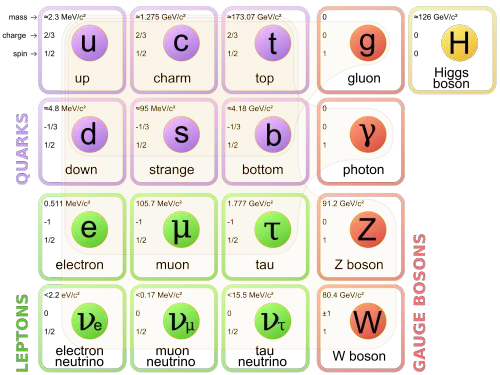
\includegraphics[width=0.84\textwidth]{ANTECEDENTES/standard_model.png}
    \caption{Clasificación de las partículas según el modelo estándar de las partículas elementales}
    \label{fig:estandard_model}
\end{figure}

Las partículas elementales están divididas en dos categorías: los fermiones y los
bosones; los fermiones están a su vez divididos en quarks y leptones los cuales tienen un valor fraccional de espín (1/2), además de que obedecen la estadística de FermiDirac y el principio de exclusión de Pauli. Los quarks son partículas elementales que constituyen a los hadrones, ya que debido al principio de confinamiento los quarks no pueden co-existir en estado libre.

Cuatro son las fuerzas fundamentales en la naturaleza: la fuerza electromagnética, la débil, la fuerte y la gravitacional. El modelo estándar incluye las tres primeras, la gravitacional no está incluida pero su contribución en la física de partículas es despreciable si se compara por ejemplo con la fuerza electromagnética (una razón de $10^{36}$ en la escala de los Giga-electrón volts). 

El modelo estándar está respaldado por una serie de observaciones experimentales, la más reciente fue la observación de una nueva partícula cuyas propiedades son consistentes con el bosón de Higgs~\cite{higgs}. Sin embargo, aún existen fenómenos en la naturaleza que no pueden ser explicados dentro del formalismo del modelo estándar, ejemplo de ello es la naturaleza y composición de la materia oscura.

\section{Materia oscura}

La materia oscura, o dark matter (por su nombre en inglés), recibe este nombre
debido a que no emite radiación electromagnética, por lo que su existencia se infiere de su influencia gravitacional sobre la materia visible (o también conocida como bariónica) que se encuentra a su alrededor; dicho fenómeno ha sido observado en cúmulos de galaxias en donde la velocidad de rotación de las mismas no corresponde a la que sería producida debido a la fuerza de gravedad ejercida por la materia visible a su alrededor.

A pesar de los esfuerzos por parte de la comunidad científica hasta este momento se desconoce la composición de la materia oscura, lo que se sabe, por medio de observaciones astronómicas, es que aproximadamente la materia oscura representa el 30.1\% de la composición materia-energía del universo, el resto es energía oscura (69.4\%) y materia visible (0.5\%). Recientemente, con el afán de entender la composición de la materia oscura y su localización en el universo, la comunidad científica ha desarrollado varios experimentos, uno de los más significativos es el Alpha Magnetic Spectrometer (AMS-02) el cual es un detector de partículas que tiene como uno de sus objetivos primordiales el de buscar indicios de materia oscura, dicho detector fue diseñado y construido en el CERN para su futura instalación en la estación espacial internacional (ISS por sus siglas en inglés). Entre sus observaciones más recientes \cite{ams:cern} se ha reportado un flujo de positrones anómalo que tiene una posible explicación en el proceso de aniquilación de partículas de materia oscura, donde se libera energía en forma de positrones. Dicho flujo anómalo puede observarse
a partir de los 25 GeV en la Figura \ref{fig:AMS_positronflux} donde también se presenta una comparación con otros experimentos que observan similar comportamiento.

\begin{figure}
    \centering
    \includegraphics[width=0.84\textwidth]{ANTECEDENTES/AMS_positronflux.png}
    \caption{Flujo de positrones medido por el experimento AMS-02, comparado con los experimentos PAMELA, Fermi-LAT, MASS, CAPIRCE, AMS-01 y HEAT.}
    \label{fig:AMS_positronflux}
\end{figure}

Estas observaciones cosmológicas han motivado a los físicos teóricos de altas energías a postular nuevos modelos en los cuales la composición de la materia oscura se pueda entender por medio de nuevas partículas elementales no descritas en el modelo estándar y que sin embargo podrían estar siendo producidas en los aceleradores de partículas modernos como el Gran Colisionador de Hadrones en Ginebra, Suiza. Los modelos propuestos se encuentran en la categoría que se conoce como extensiones al modelo estándar y por lo general involucran la existencia de nuevas partículas cuyas fuerzas e interacciones están descritas por alguna variación de la teoría cuántica de campo, lo que sugiere que sus mecanismos de producción y propiedades pueden ser estudiados por el formalismo de la física de partículas y la parte experimental por medio de los detectores de partículas con métodos de recolección de datos, selección de eventos y técnicas estadísticas para el análisis y extracción de posibles señales.

\section{Experimento CMS del CERN}

El experimento considerado en este proyecto es el Compact Muon Solenoid (CMS), el cual es uno de los detectores multi-usos del CERN que tiene la capacidad de cubrir un amplio rango de procesos físicos, reportando la observación de la partícula de Higgs en el 2012. Este experimento consiste de varios subsistemas los cuales están diseñados para la identificación de prácticamente todas las partículas del modelo estándar. Para su diseño se tomó en cuenta cómo cada partícula interacciona con la materia, por ejemplo las partículas cargadas son identificadas por medio de detectores a base de silicio y de gas noble, permitiendo determinar con precisión el tiempo y localización de las partículas, así como el signo de la carga de acuerdo a la deflexión de su trayectoria debido al poderoso campo magnético solenoide de 4 Teslas que envuelve al CMS. Las partículas neutras son identificadas por la energía que depositan en los calorímetros. La variedad de interacciones por tipo de partícula se puede ver en la Figura \ref{fig:cms_interaction}

\begin{figure}
    \centering
    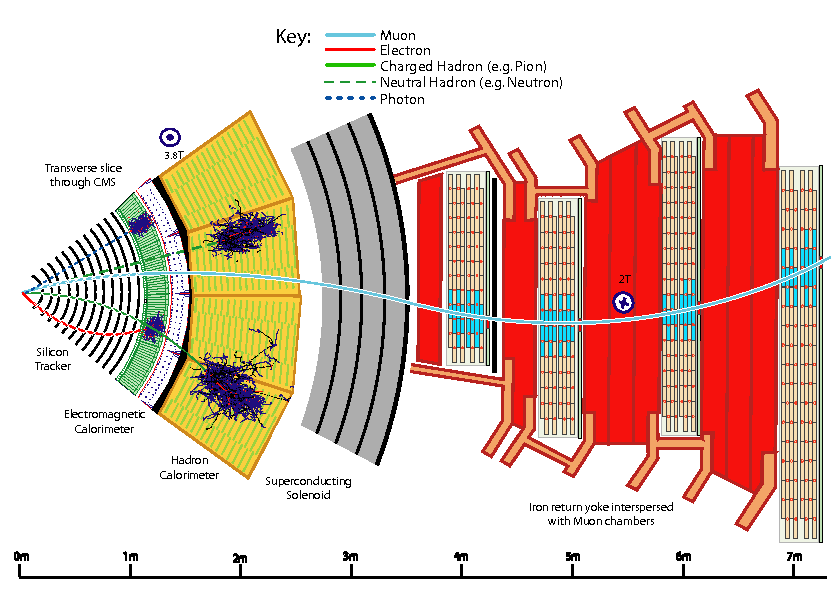
\includegraphics[width=0.84\textwidth]{ANTECEDENTES/CMS_interaction.png}
    \caption{Representación de la interacción de las partículas en el detector CMS del CERN.}
    \label{fig:cms_interaction}
\end{figure}

Los muones son partículas que interaccionan débilmente con la materia por lo que su detección se da en dos subsistemas: el detector de trazas, que corresponde a la primera capa de CMS y el sistema de muones, última capa del detector, lo cual permite una reconstrucción de trayectoria muy precisa. Debido a esto el posible decaimiento de las nuevas partículas a muones resulta en un canal favorecido desde el punto de vista experimental.

\section{Supersimetría}

Supersimetría (o SUSY por sus siglas en inglés) es una de las teorías más populares que postulan la existencia de física más allá del Modelo Estándar de Física de Partículas (teoría que describe las partículas elementales y sus interacciones). El Modelo Estándar se construye a partir de simetrías muy fundamentales que dan lugar a leyes de conservación: SUSY incluye todas las simetrías que ya contiene el Modelo Estándar y añade otra más que involucra al espín, una propiedad de las partículas elementales que hace referencia a su momento angular intrínseco.

Lo que postula SUSY es que a cada partícula del Modelo Estándar le corresponde un compañero supersimétrico que tiene el espín contrario. Es decir, por cada fermión, SUSY añade un bosón y por cada bosón añade un fermión. Por tanto, el número de partículas predicho por SUSY es el doble que en el Modelo Estándar.

\begin{figure}
    \centering
    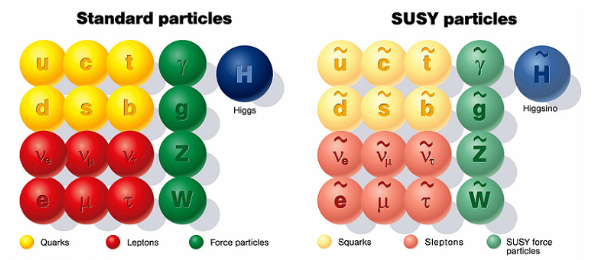
\includegraphics[width=0.84\textwidth]{ANTECEDENTES/supersimetrias.png}
    \caption{Representación de las particulas supersimétricas.}
    \label{fig:cms_interaction}
\end{figure}

Existe una relación estrecha entre SUSY y la materia oscura, en la mayoría de modelos de supersimetría (es una teoría de la que existen muchas variantes, cada una de las cuales predice fenomenologías diferentes), la partícula supersimétrica más ligera (en inglés LSP: lightest supersymmetric particle) es necesariamente neutra y estable. Esto significa que nuestro Universo estaría lleno de estas partículas masivas, neutras y estables, que por tanto serían buenas candidatas a formar la materia oscura.

Si se llega a verificar la existencia de SUSY y se consigue medir la masa de la LSP seremos capaces de decir mucho más sobre si con SUSY es suficiente para explicar la materia oscura o si se necesita algo más.























\chapter{Propuesta}

El presente trabajo se propone hacer un estudio, por medio de simulación de Monte Carlo, de los modelos teóricos que predicen la creación de nuevas partículas como producto de la colisión de protones altamente energéticos. Estas nuevas partículas serían candidatas a explicar la composición de la materia oscura. Usualmente en dichos modelos las nuevas partículas interaccionan débilmente con el sector del modelo estándar, es decir con la materia visible, por lo que su detección se dará de forma indirecta, o en otras palabras, por su decaimiento a partículas conocidas del modelo estándar []. Adicionalmente al estudio de los modelos teóricos se pretende trabajar en la parte experimental, la cual consiste en el estudio de la respuesta del detector al paso de las partículas elementales y la extracción de los observables experimentales como son la energía de las partículas, el momento y la trayectoria, entre otros. La parte experimental es fundamental ya que sin una buena estrategia de selección de datos, técnicas de supresión de ruido y optimización de la señal sería imposible la observación de esta nueva física. En este proyecto se considera el detector CMS del CERN como el aparato experimental que proporcionará los datos de estudio, ya sea por simulación o por uso de datos reales.


En una primera fase se pretende analizar los modelos teóricos de una manera fenomenológica, es decir por medio de paquetes de simulación propios del área de altas energías, además de entender la respuesta del detector a las nuevas señales buscando optimizar la selección de los eventos en base a las propiedades de cada modelo. En una segunda fase se pretende estudiar la señal de dichos modelos bajo diferentes escenarios del detector CMS, un primer escenario sería la configuración actual del detector CMS, que es la configuración usada hasta el 2018, durante el llamado período 'Run-2' y comparar los resultados con el detector que se tiene propuesto para la fase de alta luminosidad o también llamada Phase-2, la cual empezará a partir del 2025; de esta manera se puede predecir en base a los estudios de simulación las posibilidades de identificación de una nueva señal en los próximos años y cómo la actualización de los detectores y métodos de identificación de
partículas podrían contribuir a incrementar las probabilidades de descubrimiento de estas nuevas partículas.


\chapter{Justificación}

Los estudios de nueva física, en particular los que predicen la producción de nuevas partículas, son bastantes relevantes dado que se aproxima la etapa de alta luminosidad del Gran Colisionador de Hadrones en donde se logrará acumular datos con una frecuencia 10 veces mayor en la que se estaba operando. Lo anterior indica que la probabilidad de detección de nuevas señales será mucho mayor ya que se logrará alcanzar un rango de energía mayor y una cantidad de datos igualmente superior. Usualmente la probabilidad de producción de estas partículas exóticas es baja por lo que se requiere de una cantidad grande de datos para poder observar dicha producción. El período de alta luminosidad está programado para empezar a partir del año 2024 o 2025, como se puede ver en al línea de tiempo del Gran Acelerador de Hadrones en la Figura \ref{fig:LHC_timeline}, sin embargo desde este momento se está trabajando en la actualización del detector, en métodos de análisis y en estrategias que ayuden a optimizar la búsqueda de nueva física.

\begin{figure}
    \centering
    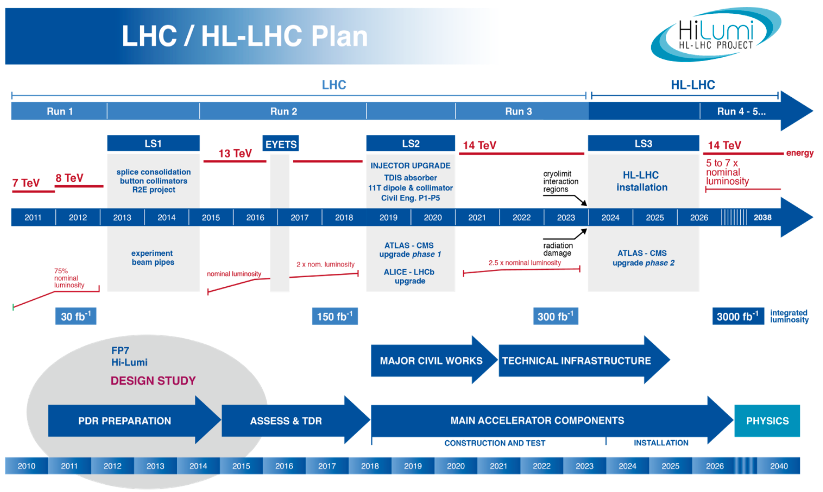
\includegraphics[width=0.84\textwidth]{JUSTIFICACION/LHC_timeline.png}
    \caption{Agenda de actividades del Gran Colisionador de Hadrones, donde la fase de alta luminosidad está programada para iniciar a partir del 2024-2025.}
    \label{fig:LHC_timeline}
\end{figure}

Actualmente los modelos teóricos que predicen la formación de partículas de materia oscura no han sido explorados ampliamente, en gran medida por falta de datos experimentales que permitan alcanzar el espacio fase que dichos modelos predicen para esas partículas. Por todo ello el funcionamiento del Gran Acelerador de Hadrones y sus proyecciones en cuanto a recolección de datos en los próximos años constituye una oportunidad perfecta para explotar con mayor intencionalidad el estudio de dichos modelos en aras de descubrir una nueva señal de fácil interpretación en el contexto de los modelos propuestos. 



\chapter{Hipótesis}

%La hipótesis que se maneja en este estudio se basa en la suposici\'on de que la materia oscura está compuesta de partículas elementales las cuales pueden ser producidas en los laboratorios modernos de física de part'iculas. De ser esto cierto se requiere de un nuevo marco teórico, es decir una extensión al modelo estándar que sustente dicha hipótesis. Afortunadamente ya se cuenta con modelos bien fundamentas que predicen dicha producción, uno de los modelos más populares es el conocido como "dark SUSY"~\cite{} en el cual existe un llamado sector oscuro donde por medio del rompimiento del grupo de simetría $U(1)_{D}$ se da lugar a la creación de fotones oscuros ($\gamma_{D}$) ligeros, los cuales interactuarían con partículas del modelo estándar y dicha fuerza de interaccion estaria descrita por medio de un parametro de mezcla cinetico $\epsilon$.  Una representacion grafica entre el sector oscuro y el del modelo estandar representa en la la Figura~\ref{fig:sketch_darksector} (izquierda). En "dark SUSY" ademas de particulas de materia oscura se da lugar a la producccion de particulas supersimetricas (SUSY), en donde la mas ligera de estas, el neutralino, dejaria de ser estable y podria decaer al foton oscuro. Las nuevas fuerzas en "dark SUSY" estarian mediadas mediante un termino de acoplamiento a la hypercarga del modelo estandar, descrito por la siguiente ecuacion.  

Si se hace supuesto que la materia oscura está compuesta de partículas elementales las cuales pueden ser producidas en los laboratorios modernos de física de partículas. De ser esto cierto se requiere de un nuevo marco teórico, una extensión al modelo estándar que sustente dicha hipótesis y el modelo conocido como "dark SUSY"~\cite{susy} en el cual predice un llamado sector oscuro donde por medio del rompimiento del grupo de simetría $U(1)_{D}$ se da lugar a la creación de fotones oscuros ($\gamma_{D}$) ligeros, los cuales interactuarían con partículas del modelo estándar y dicha fuerza de interacción estaría descrita por medio de un parámetro de mezcla cinético $\epsilon$.  Una representación gráfica entre el sector oscuro y el del modelo estándar representa en la la Figura~\ref{fig:sketch_darksector} (izquierda). En "dark SUSY" además de partículas de materia oscura se da lugar a la producción de partículas supersimétricas (SUSY), en donde la mas ligera de estas, el neutralino, dejarían de ser estable y podría decaer al fotón oscuro. 

Las nuevas fuerzas en "dark SUSY" estarían mediadas mediante un término de acoplamiento a la hipercarga del modelo estándar, descrito por la lagrangiana \cite{bb38,bb39}.

\begin{equation} 
L_{KM} = \frac{\epsilon}{2} F_{\mu\nu}^{\gamma}F^{D_{\mu\nu}}
\end{equation}

\begin{figure}
    \centering
    \includegraphics[width=0.4\textwidth]{HIPOTESIS/sketch_darksector.png}
    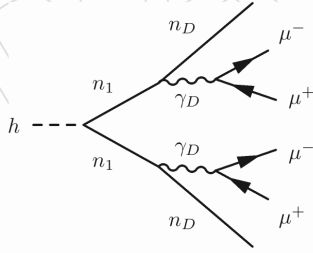
\includegraphics[width=0.4\textwidth]{HIPOTESIS/darksusy_feynman.png}
    \caption{. Ilustración esquemática de la conexión entre el sector oscuro y el modelo estándar, los cuales están conectados mediante un término de mezcla dinámica.}
    \label{fig:sketch_darksector}
\end{figure}

Donde $F_{\mu\nu}^{D}$ representa el campo oscuro y $\epsilon$ es un parámetro constante relacionado con la interacción.  De esta manera se obtiene como el fotón oscuro puede decaer a leptones \cite{bb41} del modelo estándar con una amplitud de decaimiento dada por:

\begin{equation}
  \Gamma_{\gamma D \rightarrow ll} = \frac{1}{3}\alpha \epsilon^{2} m_{\gamma D} \sqrt{1-\frac{4 m_{l}^{2}}{m_{\gamma D}^2}}(1+\frac{2m_{l}^{2}}{m_{\gamma D}}^{2})
\end{equation}

La expresión para las amplitudes permite calcular el tiempo de vida del fotos oscuro dado por: 

\begin{equation}
  \tau_{\gamma D}= \frac{\hbar}{\Gamma_{\gamma D Total}}=\frac{1}{\Gamma_{\gamma D \rightarrow e^{+}e^{-}}  + \Gamma_{\gamma D \rightarrow \mu^{+}\mu^{-}} + \Gamma_{\gamma D \rightarrow hadrons}}
\end{equation}

%%% EScribir la ecuacion. 




El diagrama de Feynman para el proceso del modelo "dark SUSY" $h\rightarrow 2n_{1}\rightarrow 2n_{D}\rightarrow 2\gamma_{D} \rightarrow 2n_{D} + 4\mu$ se muestra en la figura~\ref{fig:sketch_darksector} (derecha), el estudio de este proceso y la obtención de sus características (ver Figura \ref{fig:foton_oscuro}) permitiría inicializar escenarios extendidos de "dark SUSY" para estudios con versiones mas complejas que involucrarían otras partículas del sector oscuro como Higgs oscuros, o bosones Z y W oscuros, dando cabida a procesos como $pp\rightarrow h \rightarrow Z_{D}Z/Z_{D}Z_{D}/Z_{a}\rightarrow 4\mu$. %Sin embargo dichos modelos escapan a los alcances de esta tesis y podrian ser explorados en un analsis futuro. 

%Este escenario simple "dark SUSY" podria ser extendido de diversas maneras para estudios posteriores, como por ejemplo, en versiones mas complejas que involucrarían otras partículas del sector oscuro como Higgs oscuros, o bosones Z y W oscuros, dando cabida a procesos como $pp\rightarrow h \rightarrow Z_{D}Z/Z_{D}Z_{D}/Z_{a}\rightarrow 4\mu$. %Sin embargo dichos modelos escapan a los alcances de esta tesis y podrian ser explorados en un analsis futuro. 

\begin{figure}[h]
    \centering
   % \includegraphics[width=0.4\textwidth]{HIPOTESIS/sketch_darksector.png}
    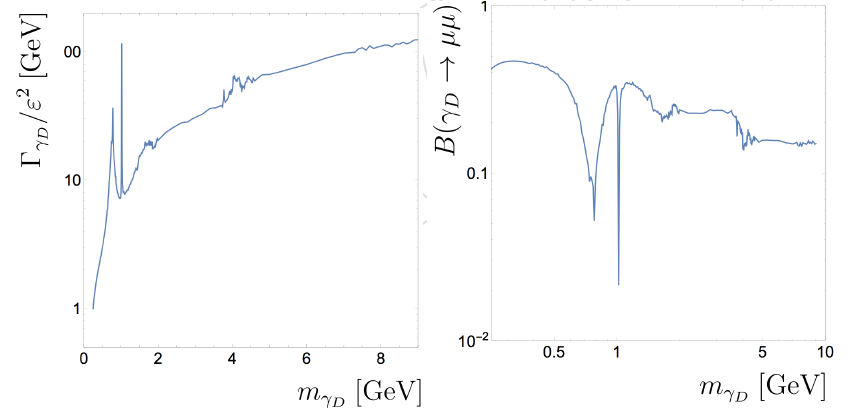
\includegraphics[width=0.8\textwidth]{HIPOTESIS/foton_oscuro.png}
    \caption{Izquierda: Peso total de los diferentes modos de desintegración del fotón oscuro, normalizado por $\epsilon^2$. Derecha: Probabilidad de decaimiento para $\gamma_D = \mu \mu$.}
    \label{fig:foton_oscuro}
\end{figure}

















\chapter{objetivo general}

El objetivo general del proyecto es que se estudie, por medio de simulación de Monte Carlos el modelo teórico "dark Susy", mediante la obtención teórica de las propiedades del fotón oscuro en un entorno simulado de los detectores que realizarían esta detección en dos configuraciones ya conocidas del experimento CMS, en la llamada fase-2 y en la de alta luminosidad.

%El objetivo general del proyecto el estudio de un modelo bien fundamentado de produccion de particulas de materia oscura. Se pretende la implementacion de dicho modelo es paquetes de simulacion propios del area de altas energias.  Caracterizacion de los parametros de dicho modelo, lo cual incluye propiedades del foton oscuro como lo son, el tiempo de vida, masa invariante, modos decaimiento, entre otros.  Adicionalmente se pretende el analisis de la respuesta del detector a dichas senales hipoteticas, tratando de extraer eficiencias de deteccion, resoluciones y metodos de supresion de ruido.  Finalmente se busca analizar las posibilidaddes de observacion de dicha particula usando la configuracion actual del detector CMS del CERN y la configuracion futura en la llamada fase-2 o de alta luminosidad. 



\chapter{Ojetivos específicos}

Los siguientes objetivos específicos a alcanzar los siguientes:
\begin{itemize}
\item Caracterizar el modelo "dark SUSY" por medio de su implementación en paquetes de simulación de altas energía, lo anterior requiere del manejo de paquetes propios de altas energías como lo son FeynRules, Madgraph, Pythia y Delphes.
\item Extracción de propiedades del modelo como lo son las propiedades básicas del fotón oscuro, masa, tiempo de vida, modos de decaimientos. %Lo anterior para verificar las  predicciones del modelo teórico.
\item Desarrollo de códigos de análisis que permitan extraer la eficiencia de detección de las partículas producidas del decaimiento del fotón oscuro, el trabajo se centrara en estudiar el decaimiento a pares de muones de signo opuesta, exploración de propiedades como función de tiempo de vida del fotón oscuro y optimización de la selección de eventos.
%\item Optimización de la selección de eventos usando como referencia las características del modelo, implementando cortes en umbrales de energía, masa, tiempo de vida propios del fotón oscuro buscando suprimir la contribución de procesos de ruido del modelo estándar. 
\item Comparación de los resultados obtenidos usando dos diferentes configuraciones del detector CMS, la actual configuración (usada hasta 2018) y la futura configuración (fase de alta luminosidad).% buscando caracterizar por medio de simulación la posible mejora en la señal con las futuras acutalizaciones del experimento CMS. 

%%%%%%%%%%% ORIGINAL CONTENIDO %%%%%%%%%%%%
%\item Caracterizar el modelo "dark SUSY" por medio de su implementación en paquetes de simulación de altas energía, lo anterior requiere del manejo de paquetes propios de altas energías como lo son FeynRules, Madgraph, Pythia y Delphes.
%\item Extracción de propiedades del modelo como lo son las propiedades básicas del fotón oscuro, masa, tiempo de vida, modos de decaimientos. Lo anterior para verificar las  predicciones del modelo teórico.
%\item Estudio de la parte experimental, desarrollo de códigos de analisis que permitan extraer la eficiencia de detección de las particulas producidas del decaimiento del foton oscuro, el trabajo se centrara en estudiar el decamiento a pares de muones de signo opuesta, exploracion de propiedades como funcion de tiempo de vida del foton oscuro
%\item Optimizacion de la seleccion de eventos usando como referencia las caracteristicas del modelo, es decir implementar cortes en umbrales de energia, masa, tiempo de vida propios del foton oscuro buscando suprimir la contribucion de procesos de ruido del modelo estandar 
%\item Comparar los resultados obtenidos usando diferentes configuraciones del detector CMS, en particular comparando la actual configuracion (usada hasta 2018) y la future configuracion (fase de alta luminosidad) buscando caracterizar por medio de simulacion la posible mejora en la senal con las futuras acutalizaciones del experimento CMS. 
\end{itemize}

\chapter{Metodología}

Con el fin de alcanzar los objetivos planteados se plantea la siguiente secuencia de actividades:


\begin{itemize}
    \item Producción de muestras de Monte Carlo (2 meses): Se espera implementar el modelo "dark SUSY" usando los paquetes propios del area y producir muestras de simulación para el proceso de senal. Las muestras se producirán usando los recursos computacionales de la Universidad de Sonora. Este paso requiere del desarrollo de código para la distribución de las corridas de simulación en forma paralela usando el cluster ACARUS. Los paquetes de simulación que se usarán serán FeynRules, MADGRAPH [], Pythia y Delphes [].
    \item Análisis preliminar (2 meses): El estudiante debe desarrollar diferentes herramientas de análisis de datos con el fin de acceder a los datos producidos en la simulación y extraer las variables de interés como lo son las propiedades del foton oscura (masa, tiempo de vida, etc.). Comúnmente dichas herramientas de análisis consisten en códigos escritos en lenguaje C++ y python, de esta manera el estudiante desarrollará habilidad en la manipulación de muestras de datos.
    \item Optimización de la selección de eventos (2 meses): Después del acceso de datos de simulación y variables de interés se procederá al estudio de la selección de eventos, la cual a grandes rasgos consiste en seleccionar el conjunto de variables físicas y valores que puedan optimizar el proceso de señal y reducir lo más posible la contribución del ruido.
    \item Análisis estadístico (3 meses): Se realizará un estudio estadístico en el cual se extraerán el número de eventos de señal y ruido después de la selección. De ahí se puede interpretar los resultados en base a indicadores estadísticos y concluir la probabilidad de observación con datos recolectados en los próximos años.
    \item Comparacion de los resultados obtenidos usando la configuracion actual del detector CMS y la configuracion que se utilizara en la llamada fase-2 o de alta luminosidad. 
    \item Escritura de Tesis (3 meses): Se presentará los resultados a expertos del área buscando una retroalimentación, procediéndose al mismo a la escritura del trabajo de tesis.
\end{itemize}

\chapter{Resultados esperados}

Al finalizar este estudio se espera obbtener los siguientes resultados: 
\begin{itemize}
    \item Caracterización del modelo "dark SUSY" logrando establecer las principales caracteristicas del foton oscuro a nivel basico de proceso de fisica de particulas 
    \item Implementación de un entorno de simulación, de una manera que sea práctico y reutilizable en la colaboración para futuros estudios.
    \item Desarrollo de nuevas herramientas de análisis que permitan incrementar la probabilidad de detección de este tipo de señales, con la implementación de algoritmos que contribuyan a la mejor identificación de partículas como el fotón oscuro.
    \item Mejorar los paquetes de simulación y análisis experimental ya que actualmente no se encuentran optimizados para el estudio de partículas como el fotón oscuro, las que debido a sus propiedades particulares (tiempo de vida largo) requieren de implementaciones especiales en la parte experimental.
\end{itemize}



%\listoftables

%\cleardoublepage
%
%\chapter{Antecedentes}

\section{Modelo Est\'andar}

El modelo est\'andar es el formalismo te\'orico-experimental que hasta el d\'{\i}a de hoy  describe con mayor precisi\'on las interacciones entre las part\'{\i}culas elementales y los diferentes tipos de fuerzas que experimentan las mismas. Los mayores desarrollos te\'oricos y descubrimientos experimentales que dieron forma al modelo Est\'andar se tuvieron en la segunda mitad del siglo XX con el desarrollo de la Teor\'{\i}a Cu\'antica de Campo, fruto del esfuerzo de cient\'{\i}ficos de todo el mundo los cuales a partir de los modelos te\'oricos y observaciones experimentales construyeron una clasificaci\'on de las part\'{\i}culas en base a sus propiedades fundamentales como lo son la masa, la carga el\'ectrica, el esp\'{\i}n, entre otras. Dicha clasificaci\'on se muestra en la Figura~\ref{fig:ME}. Las part\'{\i}culas elementales est\'an divididas en dos categor\'{\i}as, los fermiones y los bosones, los fermiones est\'an a su vez divididos en quarks y leptones los cuales tienen un valor fraccional de esp\'{\i}n (1/2), adem\'as de que obedecen la estadistica de Fermi-Dirac y el principio de exclusion de Pauli. Los quarks son particulas elementales que constituyen a los hadrones, ya que debido al principio de confinamiento los quarks no pueden co-existir en estado libre.

Cuatro son las fuerzas fundamentales en la naturaleza, la fuerza electromagn\'etica, la d\'ebil, la fuerte y la gravitacional, el modelo est\'andar incluye las tres primeras, la gravitacional no esta incluida dado que su contribuci\'on en la f\'{\i}sica de part\'{\i}culas es despreciable si se compara por ejemplo con la fuerza electromagn\'etica (una raz\'on de $10^{36}$ en la escala de los Giga-electr\'on volts). El modelo est\'andar esta respaldado por una serie de observaciones experimentales, la mas reciente fue la observaci\'on de una nueva part\'{\i}cula cuyas propiedades son consistentes con el boson de Higgs~\cite{higgs}. Sin embargo aun existen fen\'omenos en la naturaleza que no pueden ser explicados dentro del formalismo del modelo est\'andar, ejemplo de ello es la naturaleza y composici\'on de la materia oscura.

\begin{figure}
\begin{center}
  \includegraphics[width=3.6in]{standard-model.png}
  \caption{Clasificaci\'on de las particulas seg\'un el Modelo est\'andar de las part\'iculas elementales}
  \label{fig:ME}
\end{center}
\end{figure}


\section{Materia Oscura}

La materia oscura, o dark matter (por su nombre en ingles) recibe este nombre debido a que no emite radiaci\'on electromagn\'etica, por lo que su existencia se infiere debido a su influencia gravitacional sobre la materia visible (o tambi\'en conocida como barionica) que se encuentra a su alrededor, dicho fen\'omeno ha sido observado en c\'umulos de galaxias en donde la velocidad de rotaci\'on de las mismas no corresponde a la que seria producida debido a la fuerza de gravedad ejercida por la materia visible a su alrededor. A pesar de los esfuerzos por parte de la comunidad cient\'{\i}fica hasta este momento se desconoce la composici\'on de la materia oscura, lo que se sabe, por medio de observaciones astron\'omicas, es que aproximadamente la materia oscura representa el 30.1\%  de la composici\'on materia-energ\'{\i}a del universo, el resto es energ\'{\i}a oscura (69.4\%) y materia visible (0.5\%). Recientemente y con el af\'an de entender la composici\'on de la materia oscura y su localizaci\'on en el universo la comunidad cient\'{\i}fica ha desarrollado varios experimentos, uno de los mas significativos es el Alpha Magnetic Spectrometer (AMS-02) el cual es un detector de part\'{\i}culas que tiene como uno de sus objetivos primordial el de buscar indicios de materia oscura, dicho detector fue dise\~nado y construido en el CERN para su futura instalaci\'on en la estaci\'on espacial internacional (ISS por sus siglas en ingles). Entre sus observaciones mas recientes~\cite{ams:cern} se ha reportado un flujo de positrones an\'omalo cuyo origen podria ser explicado por el proceso de aniquilaci\'on de part\'{\i}culas de materia oscura, donde en dicho proceso se libera energ\'{\i}a en forma de positrones .  Dicho flujo an\'omalo puede observarse a partir de los 25~GeV en la Figura~\ref{fig:AMS_positron} donde tambi\'en se presenta una comparaci\'on con otros experimentos que observan similar comportamiento.

\begin{figure}
\begin{center}
 \includegraphics[width=4.0in]{AMS_positronflux.png}
  \caption{Flujo de positrones medido por el experimento AMS-02, comparado con los experimentos PAMELA,Fermi-LAT, MASS, CAPIRCE, AMS-01 y HEAT.}
 \label{fig:AMS_positron}
 \end{center}
\end{figure}

Dichas observaciones cosmol\'ogicas han motivado a los f\'{\i}sicos te\'oricos de altas energ\'{\i}as a postular nuevos modelos en los cuales la composici\'on de la materia oscura se pueda entender por medio de nuevas part\'{\i}culas elementales, las cuales no se encuentran descritas en el modelo est\'andar y que sin embargo podr\'{\i}an estar siendo producidas en los aceleradores de part\'{\i}culas modernos como el Gran Colisionador de Hadrones en Ginebra, Suiza.  Dichos modelos propuestos se encuentran en la categor\'{\i}a que se conoce como extensiones al modelo est\'andar y por lo general involucran la existencia de nuevas part\'{\i}culas cuyas fuerzas e interacciones est\'an descritas por alguna variaci\'on de la teor\'{\i}a cu\'antica de campo, lo que sugiere que sus mecanismos de producci\'on y propiedades pueden ser estudiadas por el formalismo de la f\'{\i}sica de part\'{\i}culas y la parte experimental por medio de los detectores de part\'{\i}culas. La parte experimental involucra la implementacion de m\'etodos de recolecci\'on de datos, selecci\'on de eventos y t\'ecnicas estad\'{\i}sticas para la extracci\'on de posibles se\~nales.

\section{Experimento CMS del CERN}
\label{cap:cms}

El experimento considerado en este proyecto es el Compact Muon Solenoid (CMS), el cual es uno de los detectores multi-usos del CERN, dicho detector tiene la capacidad de cubrir un amplio rango de procesos f\'{\i}sicos, como se comento anteriormente el CMS junto con el experimento ATLAS reportaron la observaci\'on de la part\'{\i}cula de Higgs en el 2012.  Este experimento consiste de varios subsistemas los cuales est\'an dise\~nados para la identifcaci\'on de pr\'acticamente todas las part\'{\i}culas del modelo est\'andar, para su dise\~no se tomo en cuenta como cada part\'{\i}cula interacciona con la materia, por ejemplo las part\'{\i}culas cargadas son identificadas por medio de detectores a base de silicio y de gasese nobles los cuales permiten determinar con precisi\'on el tiempo de cruce y localizaci\'on espacial de las part\'{\i}culas, adem\'as de que el signo de la carga es determinado deacuerdo a la deflecci\'on de su trayectoria debido al poderoso campo magn\'etico solenoide de 4 Teslas que envuelve al CMS.  Las part\'{\i}culas neutras son identificadas por la energ\'{\i}a que depositan en los calorimetros, la variedad de interacciones por tipo de part\'{\i}cula se puede ver en la Figura~\ref{fig:cms_interaction}. Los muones son part\'{\i}culas que interaccionan d\'ebilmente con la materia por lo que su detecci\'on se da un dos subsistemas, el detector de trazas, que corresponde a la primera capa de CMS y el sistema de muones, ultima capa del detector, lo cual permite una reconstrucci\'on de trayectoria muy precisa, debido a esto el posible decaimiento de las nuevas part\'{\i}culas a muones resulta un canal favorecido desde el punto de vista experimental.


\begin{figure}
\begin{center}
 \includegraphics[width=4.0in]{cms_interaction.png}
  \caption{Representaci\'on de la interacci\'on de las part\'{\i}culas en el detector CMS del CERN}
 \label{fig:cms_interaction}
 \end{center}
\end{figure}

\chapter{Propuesta}

En este trabajo se propone hacer un estudio por medio de simulaci\'on de Monte Carlo de los modelos te\'oricos que predicen la creaci\'on de nuevas part\'{\i}culas como producto de la colisi\'on de protones altamente energ\'eticos. Estas nuevas part\'{\i}culas serian candidatas a explicar la composici\'on de la materia oscura.  Usualmente en dichos modelos las nuevas part\'{\i}culas interaccionan d\'ebilmente con el sector del modelo est\'andar, es decir con la materia visible por lo que su detecci\'on se dar\'{\i}a de forma indirecta, o en otras palabras, por su decaimiento a part\'{\i}culas conocidas del modelo est\'andar~\cite{Curtin2015} .  Adicionalmente al estudio de los modelos te\'oricos se pretende trabajar en la parte experimental, la cual consiste en el estudio de la respuesta del detector al paso de las part\'{\i}culas elementales y extracci\'on de los observables experimentales como los son la energ\'{\i}a de las part\'{\i}culas, el momento, la trayectoria, entre otros.  La parte experimental es fundamental ya que sin una buena estrategia de selecci\'on de datos, t\'ecnicas de supresi\'on de ruido y optimizaci\'on de la se\~nal seria imposible la observaci\'on de esta nueva f\'{\i}sica. En este proyecto se considera el detector CMS del CERN como el aparato experimental que proporcionara los datos de estudio, ya sea por simulaci\'on o por uso de datos reales.  

En una primera fase se pretende analizar los modelos te\'oricos de una manera fenomenol\'ogica, es decir por medio de paquetes de simulaci\'on propios del \'area de altas energ\'{\i}as, adem\'as de entender la respuesta del detector a las nuevas se\~nales, buscando optimizar la selecci\'on de los eventos en base a las propiedades de cada modelo, en una segunda fase se pretende estudiar la se\~nal de dichos modelos bajo diferentes escenarios del detector CMS, un primer escenario seria la configuraci\'on actual del detector CMS, que es la configuraci\'on usada hasta el 2018, durante el llamado periodo 'Run-2'' y comparar los resultados con el detector que se tiene propuesto para la fase de alta luminosidad o tambi\'en llamada Phase-2, la cual empezara  a partir del 2025, de esta manera se puede predecir en base a los estudios de simulaci\'on las posibilidades de identificaci\'on de una nueva se\~nal en los pr\'oximos a\~nos y como la actualizaci\'on de los detectores y m\'etodos de identificaci\'on de part\'{\i}culas podr\'{\i}an contribuir a incrementar las probabilidades de descubrimiento de estas nuevas part\'{\i}culas. 


\chapter{Justificaci\'on}

Los estudios de nueva f\'{\i}sica, en particular los que predicen la producci\'on de nuevas part\'{\i}culas son bastantes relevantes dado que se aproxima la etapa de alta luminosidad del gran colisionador de hadrones, en donde se lograra acumular datos con una frecuencia 10 veces mayor en la que actualmente se esta operando, es decir la probabilidad de detecci\'on de nuevas se\~nales sera mucho mayor ya que se lograra alcanzar un rango de energ\'{\i}a mayor y una cantidad de datos igualmente superior. Usualmente la probabilidad de producci\'on de estas part\'{\i}culas ex\'oticas es baja por lo que se requiere de una cantidad grande de datos para poder observar dicha se\~nal. El periodo de alta luminosidad esta programado para empezar a partir del a\~no 2024 o 2025 como se puede ver en al linea de tiempo del Gran Acelerador de Hadrones en la Figura~\ref{fig:lhctimeline} sin embargo desde este momento se esta trabajando en la actualizaci\'on del detector, m\'etodos de an\'alisis y estrategias que ayuden a optimizar la b\'usquedas de nueva f\'{\i}sica. 

\begin{figure}
\begin{center}
  \includegraphics[width=4.0in]{lhc_timeline.png}
  \caption{Agenda de actividades del Gran Colisionador de Hadrones, donde la fase de alta luminosidad esta programada para iniciar a partir del 2024-2025}
  \label{fig:lhctimeline}
\end{center}
\end{figure}


Actualmente los modelos te\'oricos que predicen la formaci\'on de part\'{\i}culas de materia oscura no han sido explorados ampliamente, en gran medida por falta de datos experimentales que permitan alcanzar el espacio fase que dichos modelos predicen para esas part\'{\i}culas.  Actualmente con el funcionamiento del gran acelerador de hadrones y sus proyecciones en cuanto a recolecci\'on de datos en lo pr\'oximos a\~nos es la perfecta oportunidad para empezar a explotar lo mas posible el estudio de dichos modelos, para en dado caso descubir una nueva se\~nal sea f\'acil su interpretaci\'on en el contexto de alguno de los modelos propuesto.


\chapter{Hipotesis}

La hip\'otesis que se maneja en este estudio se basa en el estudio de modelos solidos que postulan que la materia oscura esta compuesta de part\'{\i}culas elementales, las cuales no han sido observadas hasta este momento, sin embargo podr\'{\i}an ser producidas en el laboratorio, de ser esto cierto se requiere de una marco te\'orico, es decir una teor\'{\i}a mas all\'a del modelo est\'andar que de sustento a dicha hip\'otesis. Afortunadamente ya existen varias modelos propuestos que predicen dicha producci\'on, uno de los modelos mas populares es el del llamado sector oscuro, o dark sector, por sus siglas en ingles, en el cual debido al rompimiento de una simetr\'{\i}a se da lugar a la producci\'on del llamado fot\'on oscuro (dark photon), dicha part\'{\i}cula seria la part\'{\i}cula portadora entre el sector oscuro y el del modelo est\'andar, es decir se comportar\'{\i}a como un boson, y la interacci\'on entre estos dos sectores se dar\'{\i}a por medio de lo que se conoce como el par\'ametro cin\'etico de mezcla (kinetic mixing parameter), usualmente abreviado como $\epsilon$~\cite{LB}, el cual mide la interacci\'on entre los dos sectores.

Una de las caracter\'{\i}sticas de esta nueva part\'{\i}cula y que la diferencia del fot\'on del modelo est\'andar es que seria masiva y que su tiempo de vida podr\'{\i}a ser significativo, es decir en esta teor\'{\i}a esta nueva part\'{\i}cula tendr\'{\i}a dos par\'ametros libres (masa y tiempo de vida), adem\'as de que su detecci\'on se dar\'{\i}a de forma indirecta, es decir por el decaimiento a part\'{\i}culas del modelo est\'andar.  Uno de los canales mas prometedores es en el que el fot\'on oscuro decae a muones. los muones son part\'{\i}culas que pueden ser identificadas y reconstruidas con gran eficacia usando el detector CMS como se comento en la secci\'on~\ref{cap:cms} por lo que la probabilidad de detecci\'on es mayor que con otros modos de decaimientos.

Adicionalmente en varios de estos modelos el boson de Higgs puede servir como portal del sector oscuro~\cite{Arcadi:2019lka}, es decir, existe la probabilidad de que uno de los decaimientos del boson de Higgs sea a part\'{\i}culas como el fot\'on oscuro, esto es valido para el boson de higgs del modelo est\'andar, es decir el recientemente observado y cuya masa es de 125~GeV, pero tambi\'en podr\'{\i}a ser valido en teor\'{\i}as que predicen mas de un boson de higgs, incluso con aquellos que postulan la existencia de part\'{\i}culas supersimetricas.




\begin{figure}
\begin{center}
  \includegraphics[width=2.8in]{sketch_darksector.png}
  \caption{Ilustraci\'on esquem\'aticas de la conexi\'on entre el sector oscuro y el modelo est\'andar, los cuales est\'an conectados mediante un termino de mezcla din\'amica $\epsilon$}
  \label{fig:AMS_positron}
\end{center}
\end{figure}


\chapter{Objetivo General}

El objetivo general del proyecto es que se estudien, principalmente por medio de simulaci\'on, los diferentes modelos te\'oricos disponibles que predicen la creaci\'on de part\'{\i}culas de materia oscura en las colisiones de protones del experimento CMS del CERN.  Se buscara optimizar los par\'ametros de los modelos y t\'ecnicos experimentales que contribuyan a la b\'usqueda de dicha se\~nal en los pr\'oximos a\~nos.   Se pretende que dicho trabajo de simulaci\'on sirva de base para un trabajo futuro mas detallado donde se incorporen t\'ecnicas mas avanzadas de estudio. 


\chapter{Objetivos Espec\'{\i}ficos}

Se pretende alcanzar los siguiente objetivos espec\'{\i}ficos: 

\begin{itemize}
\item Entender los modelos te\'oricos que predicen la formaci\'on de part\'{\i}culas nuevas candidatas a dar explicaci\'on a la materia oscura, lo cual incluye ser capaz de variar los par\'ametros e incluir dichas variaciones en paquetes de simulaci\'on propios de la comunidad de altas energ\'{\i}as. 
\item Desarrollar un entorno de simulaci\'on el cual permita generar muestras estad\'{\i}sticas que incluyan la descripci\'on del modelo, generaci\'on de eventos y simulaci\'on del paso de part\'{\i}culas por el detector CMS. 
 \item Desarrollar un entorno de an\'alisis el cual permita estudiar los eventos simulados o experimentales, el an\'alisis incluye desde el acceso de datos, selecci\'on de eventos, tecnicas de supresi\'on de ruido y t\'ecnicas de an\'alisis de se\~nales. 
\item Comparar los resultados con diferentes configuraciones del detector CMS, se pretende comparar el detector actual con el dise\~no futuro en la fase de alta luminosidad, esto es posible por medio de simulaci\'on. 
  
\end{itemize}


\chapter{Metodolog\'{\i}a}

Para lograr alcanzar los objetivos deseados se pretende seguir la siguiente secuencia de actividades con el tiempo aproximado para cada una de ellas:

\begin{itemize}
  
\item Producci\'on de muestras de MonteCarlo (2 meses): Se espera producir muestras de simulaci\'on de monte carlo para cada proceso de la se\~nal y ruido, el numero de eventos a producir depende del tipo de proceso que se este estudiando y su probabilidad de producci\'on, a probabilidad mayor numero de eventos que se necesitaran producir, las muestras se espera se produzcan usando los recursos computacionales de la Universidad de Sonora. Dicho paso requiere del desarrollo de c\'odigo para la distribuci\'on de las corridas de simulaci\'on en forma paralela usando el cluster ACARUS. Los paquetes de simulaci\'on que se usaran ser\'an MADGRAPH~\cite{Alwall:2007st}, Pythia y Delphes~\cite{deFavereau2014}.

\item An\'alisis preliminar (2 meses): El estudiante debe desarrollar diferentes herramientas de an\'alisis de datos, con el fin de acceder a los datos producidos en la simulaci\'on y extraer las variables de inter\'es, com\'unmente dichas herramientas de an\'alisis consisten de c\'odigos escritos en lenguaje C++ y python, de esta manera el estudiante desarrollar\'a habilidad en la manipulaci\'on de muestras de datos. 

\item Optimizaci\'on de la selecci\'on de eventos (2 meses): Despu\'es del acceso de datos de simulaci\'on y variables de inter\'es se proceder\'a al estudio de la selecci\'on de eventos, la cual a grandes rasgos consiste en seleccionar el conjunto de variables fisicas y valores los cuales puedan optimizar el proceso de se\~nal y reducir lo mas posible la contribuci\'on del ruido. 

\item An\'alisis estad\'{\i}stico (3 meses): Despu\'es de la selecci\'on de eventos se realizara un estudio estad\'{\i}stico en el cual se extraer\'an el numero de eventos de se\~nal y ruido desp\'ues de la selecci\'on, de ah\'{\i} se puede interpretar los resultados en base a indicadores estad\'{\i}sticos y concluir la probabilidad de obsservaci\'on con datos recolectados en los siguientes a\~nos.

\item Escritura de Tesis (3 meses): Despu\'es del an\'alisis estad\'{\i}stico se presentara los resultados con expertos del \'area buscando una retroalimentaci\'on, al mismo tiempo se proceder\'a a la escritura del trabajo de tesis. 

\end{itemize}
  
\chapter{Resultados Esperados} 

De este proyecto se espera obtener los siguientes resultados.

\begin{itemize}
\item Identificaci\'on de los modelos te\'oricos mas interesantes y cuyos par\'ametros sean accesibles con la configuraci\'on del detector CMS, es decir la energ\'{\i}a de colisi\'on y los eventos proyectados a recolectar en los proximos a\~nos, de esta manera se pretende acotar los diferentes modelos disponibles.
\item Imnplementaci\'on de un entorno de simulaci\'on, de una manera que sea practico y reutilizable por la colaboraci\'on para futuros estudios
\item Desarrollo de nuevas herramientas de an\'alisis que permitan incrementar la probabilidad de detecci\'on de este tipo de se\~nales, es decir se buscara implementar algoritmos que contribuyan a la mejor identificaci\'on de part\'{\i}culas como el fot\'on oscuro.
\item Mejorar los paquetes de simulaci\'on y an\'alisis experimental ya que actualmente no se encuentran optimizados para el estudio de part\'{\i}culas como el fot\'on oscuro, que debido a sus propiedades particulares (tiempo de vida largo) y se requiere de implementaciones especiales en la parte experimental.
\end{itemize}






%\nocite{*}
\printbibliography 


\end{document}
